\section{Computational Results}


The results presented in this section were generated using an Intel i7-10700 CPU with 8 cores at 3.30 GHz, and 16 GB of RAM. We utilised Python 3.10 within VS Code (version 1.92.2). For further details, please refer to \href{https://github.com/adasilva33/DASA_Kiwi_TSP_Challenge_2}{\faGithub\ GitHub} and \href{https://github.com/ahmedkheiri//DASA_Kiwi_TSP_Challenge_2}{\faGithub\ GitHub}. 
Simulations for each considered instance were conducted, testing various parameter combinations in the grid search defined in Table \ref{table:Grid search}. One challenge encountered was the computational budget when using Python. As a result, the size of the grid search for the more complex instances was reduced, as shown in Table \ref{table:Grid search}.

\begin{table}[h]
    \centering
    \caption{Grid search}
    \resizebox{.4\textwidth}{!}{ % Resize the table to fit the text width
        \begin{tabular}{c|c|c}
            \cmidrule(r){2-3}
                                        & ($I_1,\ldots,I_6$)        & ($I_7, I_8$)     \\
            \midrule
            \textit{selection\_policy}  & top\_k, ratio\_k          & top\_k, ratio\_k \\
            \textit{simulation\_policy} & random, greedy, tolerance & greedy           \\
            \textit{selection\_policy}  & UCB, UCB1T                & UCB              \\
            \textit{C\_p}               & 0, 1.4, 2.8               & 1.4              \\
            \textit{N\_c}               & 5, 10, 15                 & 10               \\
            \textit{Ratio c}            & 0, .3, .5, .8, 1          & .5               \\
            \textit{N° simulations}     & 10                        & 10               \\
            \bottomrule
        \end{tabular}
    }
    \label{table:Grid search}
\end{table}

After running the simulations with the grid search parameters defined in Table \ref{table:Grid search}, we compared our results with the best known solutions, as presented in Table \ref{table:Best result vs state of the art} \cite{reinforcement_learning_yaro}. Note that only a subset of problem instances was considered due to the computational complexity and time constraints associated with evaluating all possible configurations for larger instances. 

\begin{table}[h]
    \centering
        \caption{Best results vs State of the art. Solutions were found for instances $I_1$, $I_2$, $I_3$, $I_4$, $I_7$, and $I_8$}

    \resizebox{.4\textwidth}{!}{ % Resize the table to fit the text width
        \begin{tabular}{|>{\centering\arraybackslash}p{1cm}
            >{\centering\arraybackslash}p{1cm}
            >{\centering\arraybackslash}p{1cm}
            >{\centering\arraybackslash}p{1cm}
            >{\centering\arraybackslash}p{1cm}
            >{\centering\arraybackslash}p{1cm} |}
            \toprule
            Instance & Best known & Best found    & Gap (\%) & Mean & Std   \\
            \midrule
            $I_1$    & 1396       & \textbf{1396} & 0        & 1396    & 0     \\
            $I_2$    & 1498       & \textbf{1498} & 0        & 1498    & 0     \\
            $I_3$    & 7672       & \textbf{7672} & 0        & 7672    & 0     \\
            $I_4$    & 13952      & 15361         & 10.1     & 15361     & 0 \\
            $I_5$    & 690        & -             & -        &  -    & -     \\
            $I_6$    & 2159       & -             & -        & -     & -     \\
            $I_7$    & 30937      & 31924         & 3.19     & 30937    & 0     \\
            $I_8$    & 4052       & \textbf{4037} & -0.52    & 4052    & 0     \\
            \bottomrule
        \end{tabular}
    }
    \label{table:Best result vs state of the art}
\end{table}

For instances $I_1$, $I_2$, and $I_3$, solutions were found and the various simulations were carried out successfully. Consequently, we investigated the influence of the parameters on the $\mathcal{MCTS}$ function and the final solution. However, for instance $I_4$, only a few parameterisations of the $\mathcal{MCTS}$ algorithm were successful in finding a solution. Specifically, the UCB1T selection policy combined with the tolerance or random simulation policies resulted in trees that were too large to find solutions within a reasonable time frame.

\subsubsection*{Analysis on $C_p$}

\begin{figure}[!ht]
    \centering
    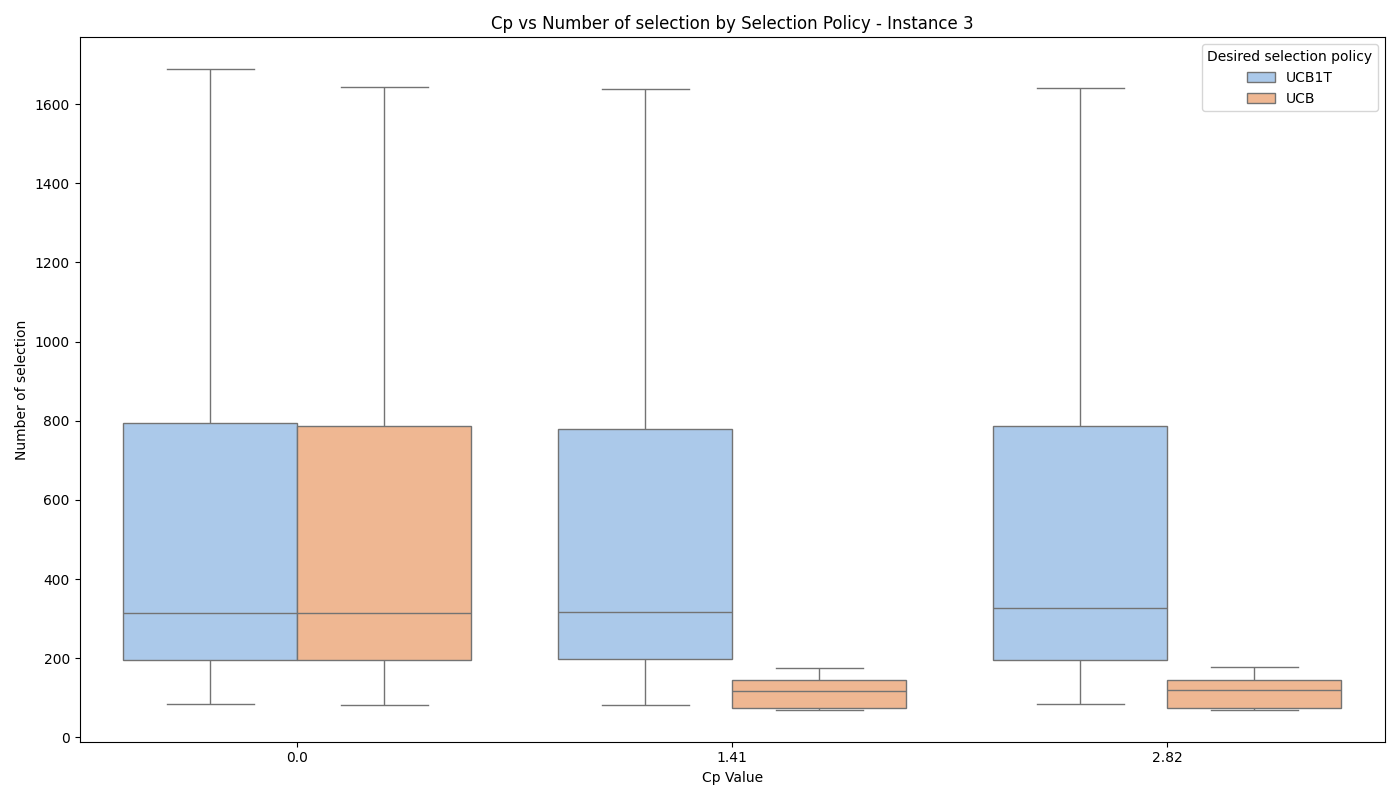
\includegraphics[width=.4\textwidth]{Figures/3 - cp_vs_selection.png}
    \caption{Effect of \(C_p\) on the Number of Selections}
    \label{fig:cp_vs_selection_3}
\end{figure}

Figure \ref{fig:cp_vs_selection_3} presents box plots illustrating the relationship between the exploration constant \(C_p\) and the number of selection phases under the UCB and UCB1T selection policies:

\begin{itemize}
    \item \textbf{\(C_p = 0\) leads to identical performance:}
          When \(C_p = 0\), the UCB and UCB1T selection policies are equivalent, resulting in identical decision-making during MCTS.
    \item \textbf{Higher \(C_p\) values lead to faster convergence for UCB:}
          As \(C_p\) increases from 0.0 to 2.82, the median number of selection phases under the UCB policy decreases.
    \item \textbf{UCB1T encourages more exploration:}
          UCB1T consistently results in a higher number of selection phases compared to UCB, particularly at higher \(C_p\) values. This aligns with UCB1T's design to promote broader exploration before converging.
\end{itemize}

While UCB1T may require more time to converge, it generally explores the search tree more effectively, leading to better overall performance. One can notice that $C_p$'s correlation with the UCB1T selection policy for $I_3$ is low.

\subsubsection*{Analysis of Expansion Ratio $c$}

When comparing the relationship between the expansion ratio (the proportion of expanded child nodes that have the cheapest flight connection among the chosen number of children) and the time required to find a solution for the UCB and UCB1T policies, several conclusions can be drawn:

\begin{itemize}
    \item \textbf{UCB finds solutions faster than UCB1T:}
          Across all expansion ratio values, the UCB policy consistently finds solutions more quickly than UCB1T. This suggests that UCB, being less aggressive in exploration, converges on solutions faster.

    \item \textbf{Higher ratios lead to faster convergence:}
          For both policies, the time to find a solution generally decreases as the expansion ratio increases. This indicates a more efficient search process when expanded nodes are less randomly chosen from the set of available actions. However, for more complex instances, maintaining a ratio \( r \in [0.3, 0.7] \) is crucial to avoid getting stuck in potential leaf nodes.
\end{itemize}

Finally, the UCB policy exhibits a stronger correlation with the expansion ratio compared to UCB1T, as shown in Figure \ref{fig:ratio_vs_cost_3}. Despite this correlation, UCB's overall performance is inferior to that of UCB1T. This is because UCB relies more heavily on exploitation, whereas UCB1T, though slower to converge, achieves better results by balancing exploration and exploitation more effectively.

\begin{figure}[!ht]
    \centering
    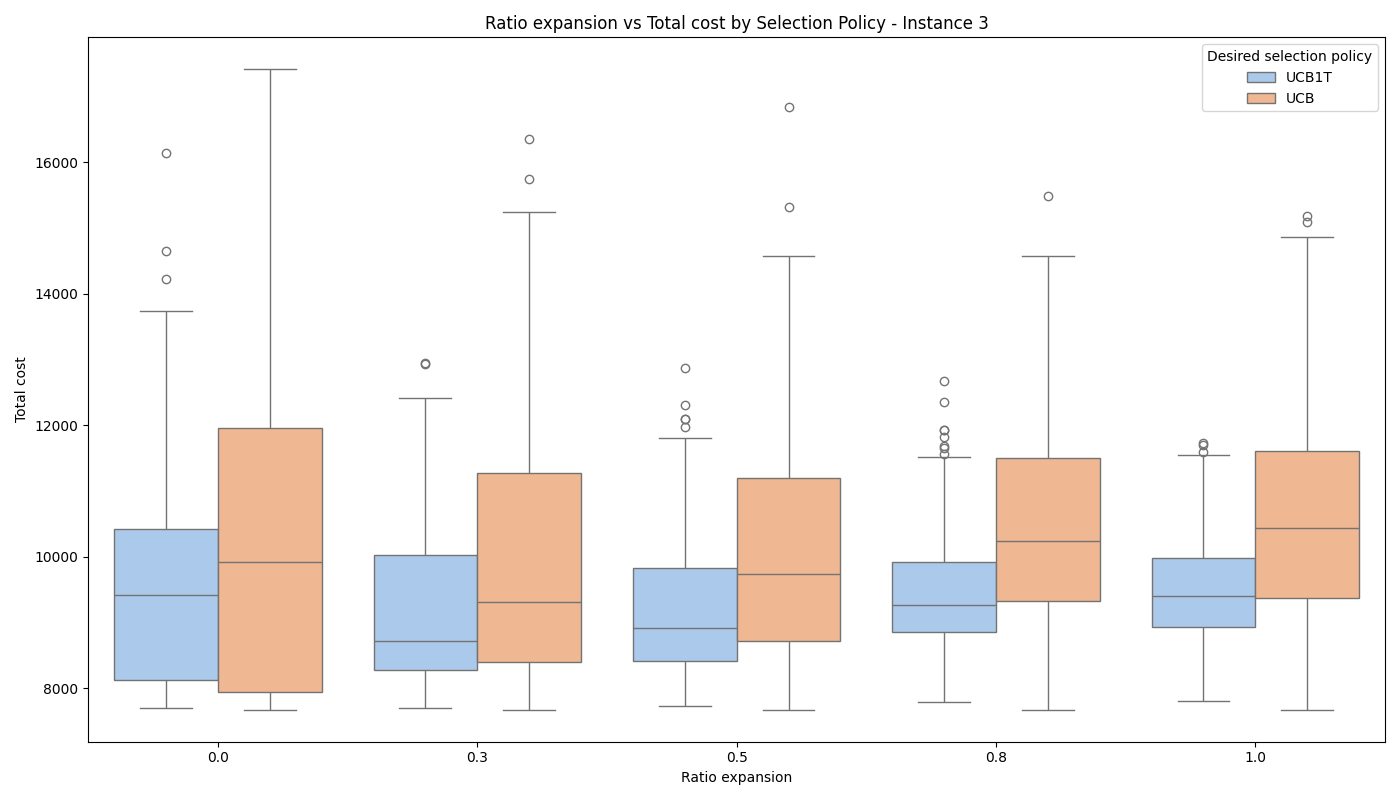
\includegraphics[width=.4\textwidth]{Figures/3 - ratio_vs_cost.png}
    \caption{Expansion ratio vs Total cost}
    \label{fig:ratio_vs_cost_3}
\end{figure}

\subsubsection*{Analysis of Simulation Performances}

\begin{figure}[!ht]
    \centering
    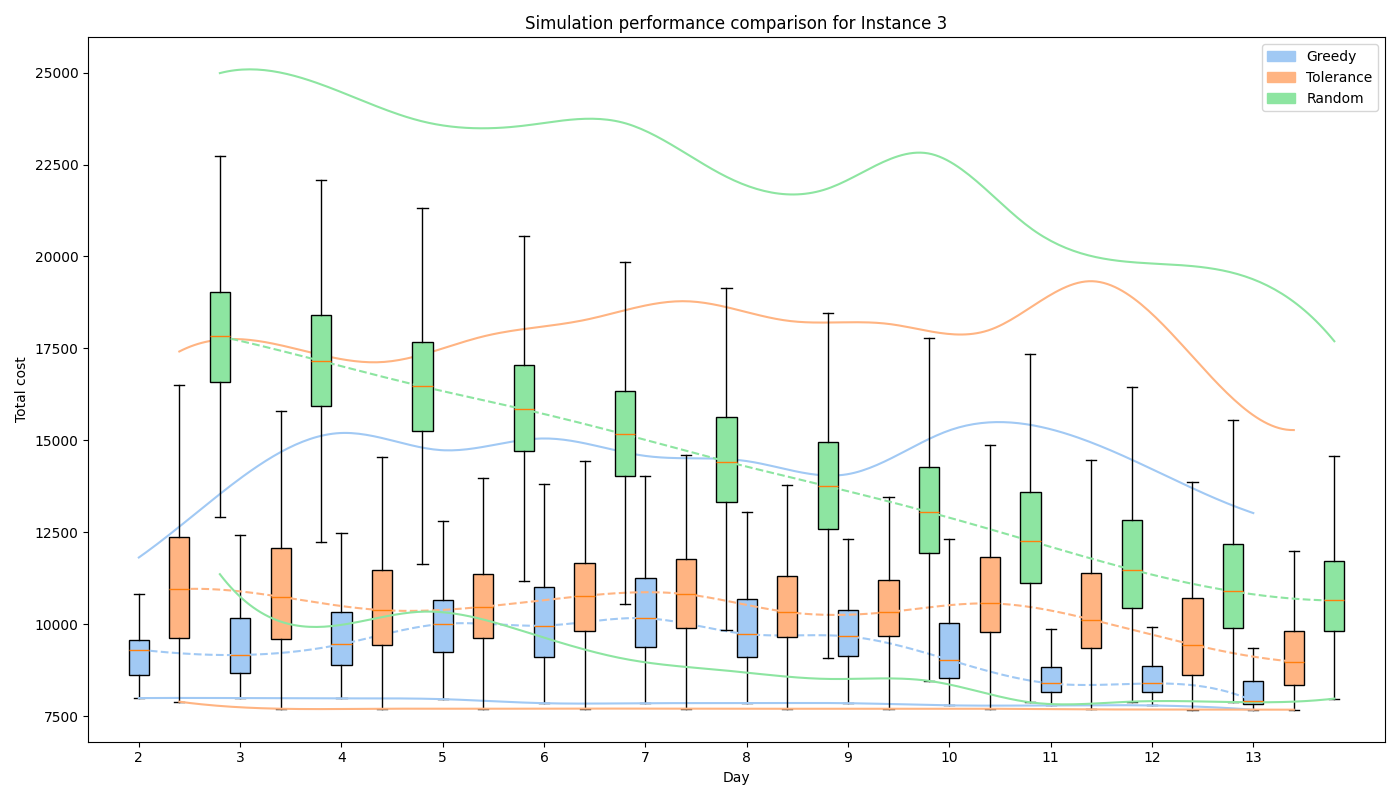
\includegraphics[width=.4\textwidth]{Figures/3 - Simulation performance.png}
    \caption{Simulation performance for Instance 3}
    \label{fig:sim_perf_3}
\end{figure}

Figure \ref{fig:sim_perf_3} presents box plots for the different simulation policies applied to Instance 3. For each day, the distribution of the simulated outcomes is plotted according to the simulation policy used. Coloured curves indicate the minimum and maximum values of these distributions, while dashed lines represent the medians.

In Figure \ref{fig:sim_perf_3}, the greedy simulation policy demonstrates superior performance, as evidenced by lower minimum, maximum, and median values of the simulation outcomes across all days. The pronounced convergence of the random policy reflects the inherent randomness of this approach. Additionally, for the greedy and tolerance policies, the minimum value is nearly reached by the second or third day of simulation. This suggests that a well-calibrated set of parameters for the $\mathcal{MCTS}$ algorithm should ideally converge towards the minimum cost observed during the simulations. If the algorithm does not achieve this, it indicates that the $\mathcal{MCTS}$ parameterisation may be suboptimal. 
Figure \ref{fig:sim_perf_vs_c_4} illustrates the distributions of simulated outcomes for a misparameterised $\mathcal{MCTS}$ instance ($I_4$). 

In Figure \ref{fig:sim_perf_vs_c_3}, the median distributions for different scenarios are plotted. The analysis reveals that values of $c$ too close to 1 do not, on average, converge to the minimum-cost solution. In contrast, lower values of $c$ tend to guide the tree search more effectively during the first days of simulations. This is crucial because it helps avoid excessive expansion of the search tree, which can lead to inefficient and time-consuming MCTS processes.

\begin{figure}[!ht]
    \centering
    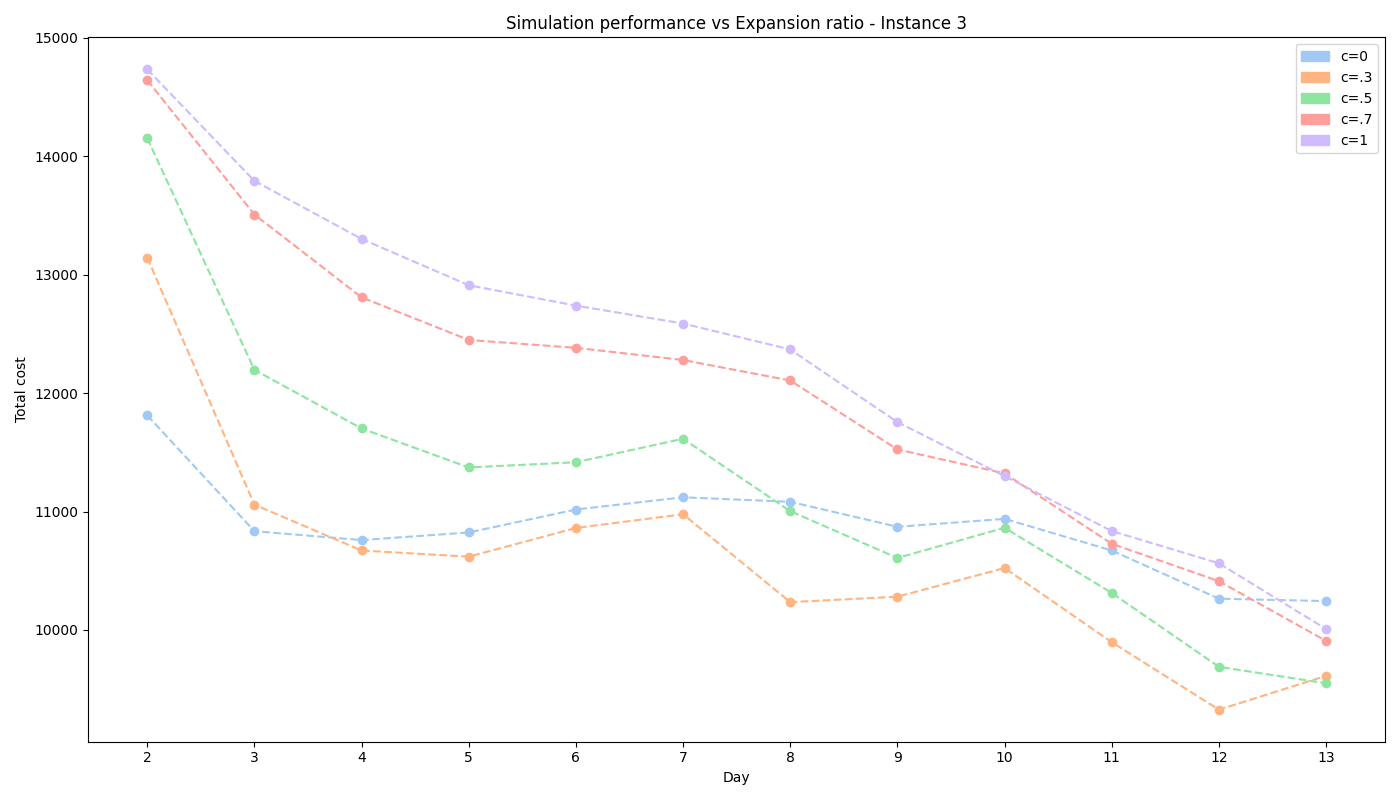
\includegraphics[width=.4\textwidth]{Figures/3 - Simulation performance vs Expansion ratio.png}
    \caption{Simulation performance vs Expansion Ratio - Instance 3}
    \label{fig:sim_perf_vs_c_3}
\end{figure}

These conclusions apply to smaller instances. However, for instance $I_4$, as shown in Figure \ref{fig:sim_perf_vs_c_4}, having $c=0$ with a greedy selection policy proves inefficient. The search tree diverges from the minimum simulated cost, resulting in the tree search failing to find a solution within 10 minutes. Based on the median comparison, $c=1$ emerges as a more optimal parameter for guiding the tree search in this case.

\begin{figure}[!ht]
    \centering
    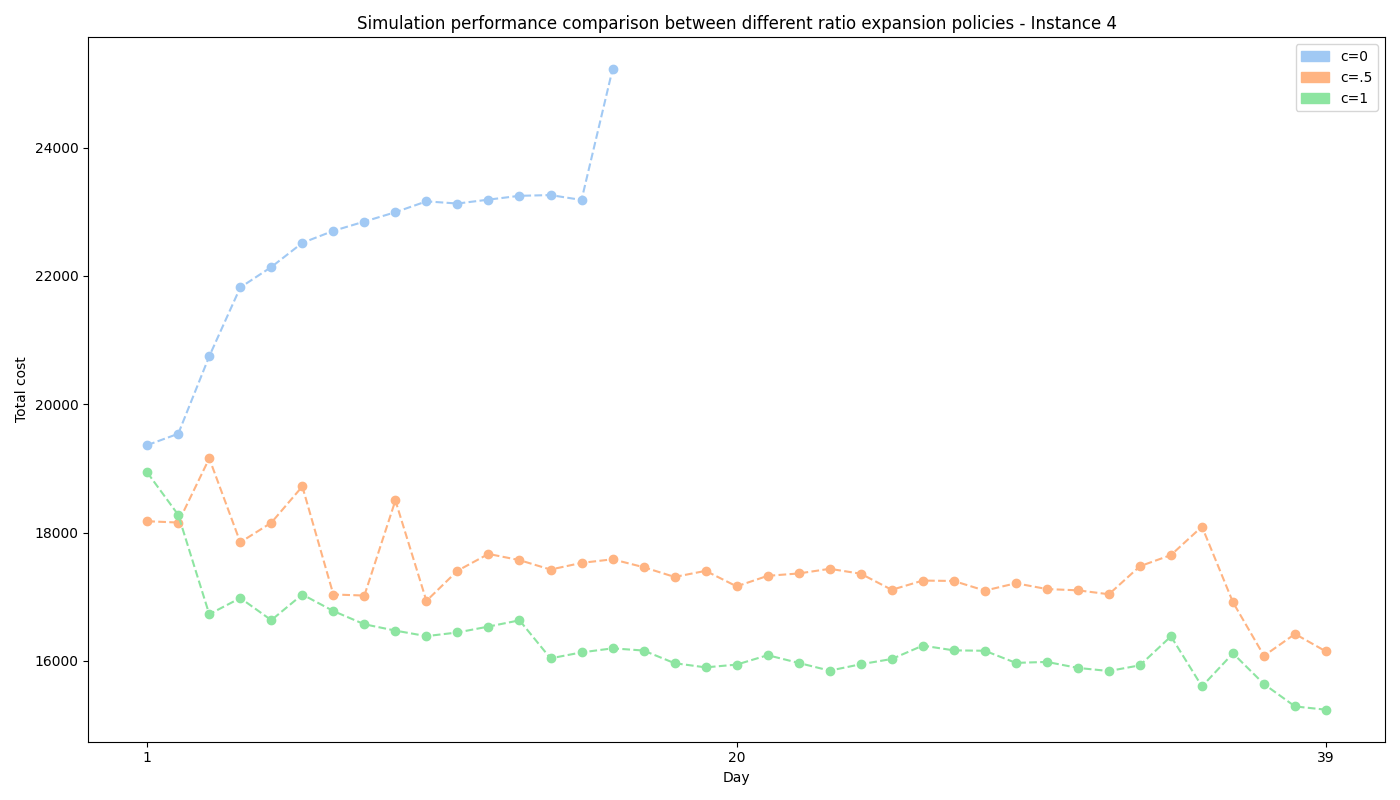
\includegraphics[width=.4\textwidth]{Figures/4 - Simulation performance vs Expansion ratio.png}
    \caption{Simulation performance vs Expansion Ratio - Instance 4}
    \label{fig:sim_perf_vs_c_4}
\end{figure}

The MCTS function struggled to effectively search the tree for instances $I_5$ and $I_6$ using grid search, as nodes simulated under random or tolerance policies that reached final states did not facilitate further tree expansion. Instances $I_7$ and $I_8$ were solved using a UCB selection policy with \(C_p = 1.41\) and \(N_c = 5\) under the top\_k expansion policy. For $I_7$, the solution found was higher by 3.19\% compared to the state of the art. In contrast, for $I_8$, a new state-of-the-art solution was achieved, improving the best known solution by 0.52\%.

\subsubsection*{Parallelisation}

In our implementation for instance $I_4$, we parallelised the MCTS across five cores. The parameters were selected to illustrate the effects of parallelisation in a stochastic environment. The parallelisation was applied during the simulation phase of the MCTS, with the minimum outcome from the five parallel simulations being chosen as the final result. In Figure \ref{fig:sim_perf_parral_4}, the distribution of outcomes from using five cores for parallelisation shows better performance compared to the non-parallelised approach. This confirms that parallelisation enhances the effectiveness of the MCTS, particularly in the initial days of the tree search.

\begin{figure}[!ht]
    \centering
    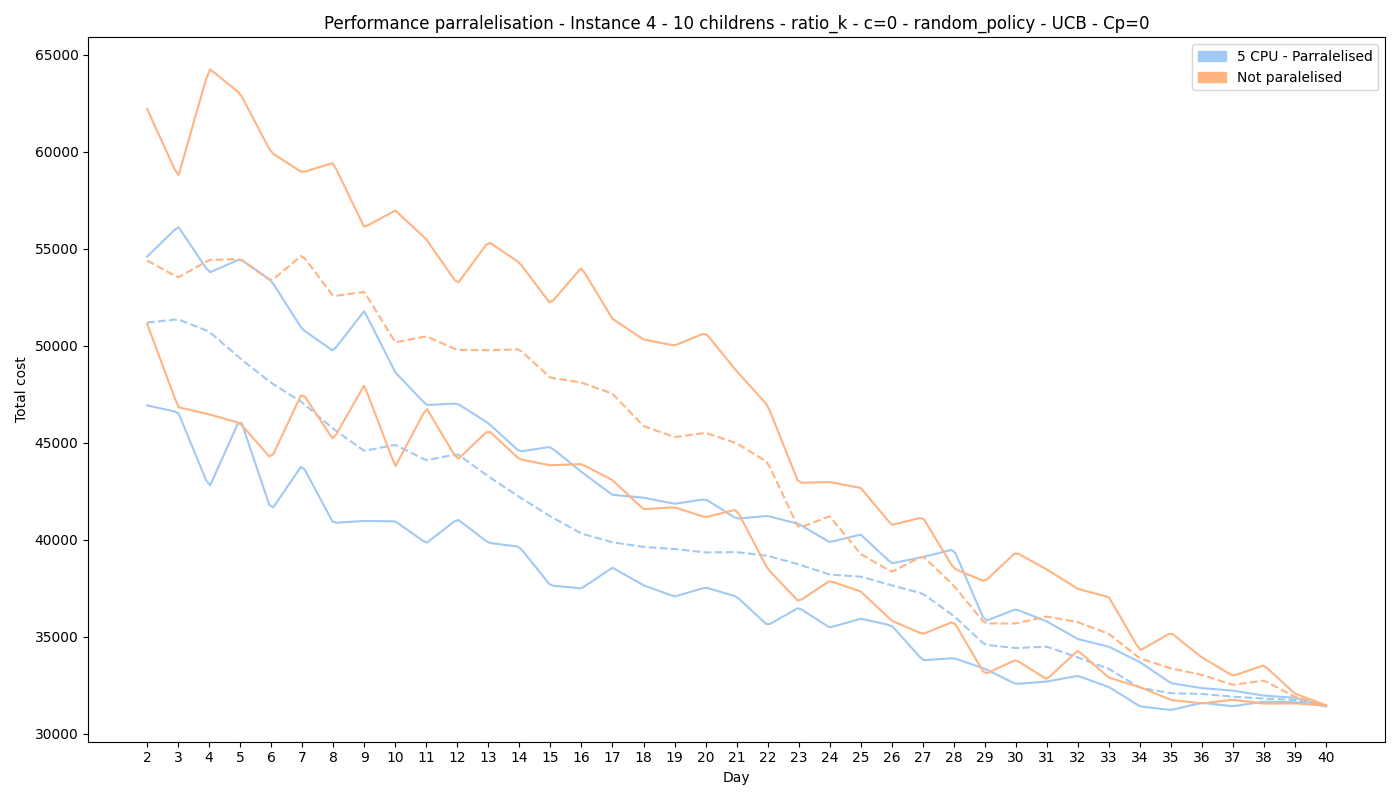
\includegraphics[width=.4\textwidth]{Figures/4 - Paralelised vs 5 CPU paralelised.png}
    \caption{Comparison of the distributions for the simulated outcomes without parallelisation and with 5 cores - Instance 4}
    \label{fig:sim_perf_parral_4}
\end{figure}


The comparative analysis of five-core and ten-core parallelisations of MCTS, evaluated using Mann-Whitney and Kolmogorov-Smirnov tests as shown in Figure \ref{fig:Stats test 5 VS 10 Parall}, revealed no statistically significant improvements at the 5\% level. As discussed in \cite{different_selection_policies}, excessive modifications to the MCTS can sometimes lead to undesirable behaviour.

\begin{figure}[!ht]
    \centering
    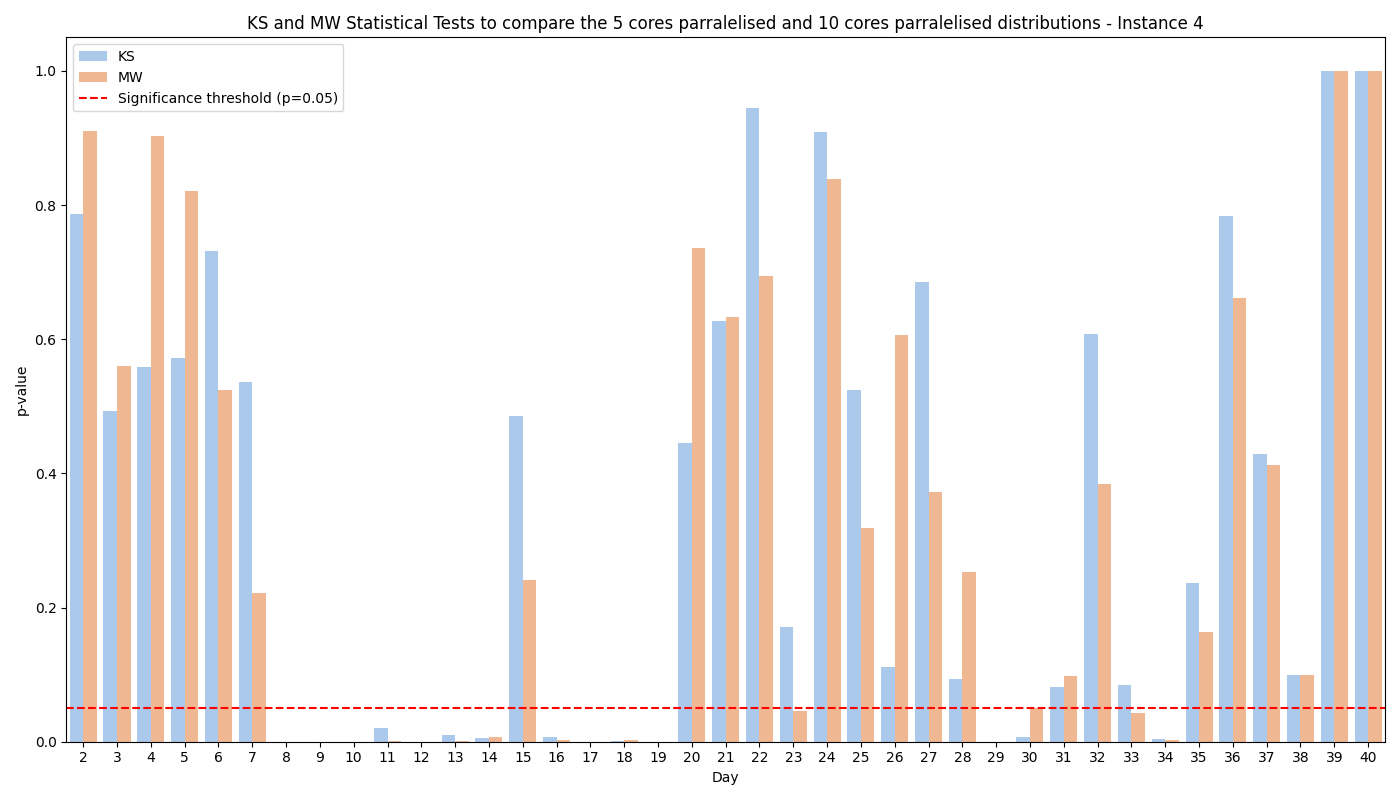
\includegraphics[width=.4\textwidth]{Figures/4 - Distribution stats tests 5P vs 10P.png}
    \caption{Statistical tests to compare the 5 \& 10 cores distribution - Instance 4}
    \label{fig:Stats test 5 VS 10 Parall}
\end{figure}
